
Let
$X_i\in\,$\cbrak{1,2,3,4,5,6}, i = 1,2,3,4  be the random variables representing the outcome for each die. As the dies are fair, the probability mass function (pmf) is expressed as
\begin{align}
    p_{X_i}(n) = \pr{X_i = n} = 
\begin{cases}
\frac{1}{6} & 1 \le n \le 6
\\
0 & otherwise
\end{cases}\label{cs2014-48:1}
\end{align}
Let X be a random variable denotes the desired outcome,
\begin{align}
    X=X_1+X_2+X_3+X_4\label{cs2014-48:2}\\
    \implies X\in\cbrak{4,5,\cdots,24}
\end{align}
We have to find $P_X(n)$ = $\pr{X_1+X_2+X_3+X_4=n}$
The Z-transform of $p_X(n)$ is defined as
\begin{align}
P_X(z) = \sum_{n = -\infty}^{\infty}p_X(n)z^{-n}, \quad z \in \mathbb{C}
\label{cs2014-48:7}
\end{align}
%
From \eqref{cs2014-48:1} and \eqref{cs2014-48:7}, 
\begin{align}
\nonumber P_{X_1}(z) =P_{X_2}(z)=P_{X_3}(z)&=P_{X_3}(z)\\
&= \frac{1}{6}\sum_{n = 1}^{6}z^{-n}
\\
&=\frac{z^{-1}\brak{1-z^{-6}}}{6\brak{1-z^{-1}}}, \quad \abs{z} > 1
\label{cs2014-48:8}
\end{align}
upon summing up the geometric progression.From convolution
\begin{align}
\because p_X(n) &= p_{X_1}(n)*p_{X_2}(n)*p_{X_3}(n)*p_{X_4}(n),
\\
P_X(z) &= P_{X_1}(z)P_{X_2}(z)P_{X_3}(z)p_{X_4}(z)
\label{cs2014-48:9}
\end{align}
The above property follows from Fourier analysis and is fundamental to signal processing.\\
From \eqref{cs2014-48:8} and \eqref{cs2014-48:9},
\begin{align}
    P_X{\brak{z}}&=\cbrak{\frac{z^{-1}\brak{1-z^{-6}}}{6\brak{1-z^{-1}}}}^4\\
    &= \frac{1}{1296}\frac{z^{-4}\brak{1-4z^{-6}+6z^{-12}-4z^{-24}+z^{-24}}}{\brak{1-z^{-1}}^4}\label{cs2014-48:10}
\end{align}
Using the fact that,\\
\begin{align}
p_X(n-k) &\system{Z}P_X(z)z^{-k},
\\
nu(n)&\system{Z} \frac{z^{-1}}{\brak{1-z^{-1}}^2}\\
n^2u(n)&\system{Z} \frac{z^{-1}\brak{1+z^{-1}}}{\brak{1-z^{-1}}^3}\\
(n^2+n)u(n)&\system{Z} \frac{2z^{-1}}{\brak{1-z^{-1}}^2}\\
(n^3+3n^2+2n)u(n)&\system{Z} \frac{6z^{-1}}{\brak{1-z^{-1}}^4}
\end{align}
\begin{figure}[htp]
    \centering
    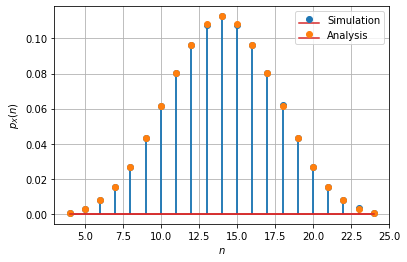
\includegraphics[width=\columnwidth]{solutions/cs/2014/48/figures/assignment4.png}
    \caption{Probability of getting sum of 22}
\end{figure}
after some algebra, it can be shown that,
\begin{multline}
\frac{1}{1296\times 6}\lsbrak{\brak{(n-3)^3+3(n-3)^2+2(n-3)}u(n-3)} \\- 4\brak{(n-9)^3+3(n-9)^2+2(n-9)}u(n-9)\\+6\brak{(n-15)^3+3(n-15)^2+2(n-15)}u(n-15)\\-4\brak{(n-21)^3+3(n-21)^2+2(n-21)}u(n-21)\\+\rsbrak{\brak{(n-27)^3+3(n-27)^2+2(n-27)}u(n-27)}
\\
\system{Z}
\frac{1}{1296}\frac{z^{-4}\brak{1-4z^{-6}+6z^{-12}-4z^{-24}+z^{-24}}}{\brak{1-z^{-1}}^4}
\label{cs2014-48:11}
\end{multline}
where 
\begin{align}
u(n) =
\begin{cases}
1 & n \ge 0
\\
0 & n < 0\label{cs2014-48:13}
\end{cases}
\end{align}
From \eqref{cs2014-48:7},\eqref{cs2014-48:10} and \eqref{cs2014-48:11},
\begin{multline}
p_{X}(n) = \frac{1}{1296\times 6}\times\\\lsbrak{\brak{(n-3)^3+3(n-3)^2+2(n-3)}u(n-3)} \\- 4\brak{(n-9)^3+3(n-9)^2+2(n-9)}u(n-9)\\+6\brak{(n-15)^3+3(n-15)^2+2(n-15)}u(n-15)\\-4\brak{(n-21)^3+3(n-21)^2+2(n-21)}u(n-21)\\+\rsbrak{\brak{(n-27)^3+3(n-27)^2+2(n-27)}u(n-27)}
\label{cs2014-48:12}
\end{multline}
From \eqref{cs2014-48:13} and \eqref{cs2014-48:12},
\begin{align}
p_X(n) &= 
\begin{cases}
0 & n < 4\\
\frac{n^3-6n^2+11n-6}{7776} &  4 \le n \le  9\\
\frac{90n^2-3n^3-753n+2010}{7776} & 9 < n \le 15\\
\frac{3n^3-162n^2+2769n-14370}{7776} & 15 < n \le 21\\
\frac{-n^3+78n^2-2027n+17550}{7776} & 21 < n \le 24\\
0 & 24 < n \label{cs2014-48:14}
\end{cases}
\end{align}
% \begin{figure}[htp]
%     \centering
%     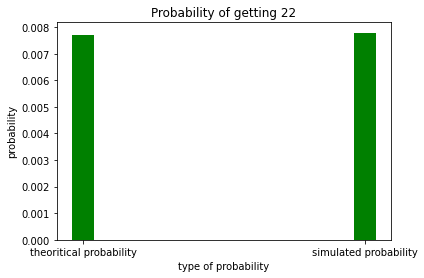
\includegraphics[width=\columnwidth]{solutions/cs/2014/48/figures/assignment4_stem.png}
%     \caption{Probability mass function of X}{ (simulations are close to analysis)}
% \end{figure}
We need probability of getting sum of 22,\\$\implies$ n=22 \\from \eqref{cs2014-48:14} and using n=22,
\begin{align}
    p_X(22)&=\frac{-(22)^3+78(22)^2-2027(22)+17550}{7776}\\
    p_X(22)&=\frac{60}{7776}\\
    p_X(22)&=\frac{10}{1296}
\end{align}